\documentclass[competition,nonblindrev, 12pt]{informs3-competition}
%\def\paperversion{1}
%\ifnum\paperversion=1
%\input{arxiv}
\newcommand{\Var}{\mathbb{V}\mathrm{ar}}
%\usepackage{xtable}
\usepackage{booktabs}
\usepackage{multicol}
\usepackage{multirow}
%        \usepackage{setspace}
\usepackage{wrapfig}

\usepackage[numbers]{natbib}
\usepackage{bm}
\usepackage{floatflt}
 \def\bibfont{\small}%
 \def\bibsep{\smallskipamount}%
 \def\bibhang{24pt}%
 \def\newblock{\ }%
 \def\BIBand{and}%
\TheoremsNumberedThrough   
\ECRepeatTheorems
\theoremstyle{TH}%
\newtheorem{condition}{Condition}
%\newtheorem{assumption}{Assumption}
\usepackage{wrapfig}
\usepackage[subtle]{savetrees}
\newcommand{\RNum}[1]{\uppercase\expandafter{\romannumeral #1\relax}}
\newcommand{\cO}{\mathcal{O}}
\newcommand{\tO}{\widetilde{\mathcal{O}}}

\newcommand*{\QED}{%
\leavevmode\unskip\penalty9999 \hbox{}\nobreak\hfill
    \quad\hbox{$\square$}%
}
\theoremstyle{TH}%
%\newtheorem{condition}{Condition}
\usepackage{booktabs}
\usepackage[font=small]{caption}
\usepackage[size=small]{subcaption}
\captionsetup[figure]{font={bf,small},skip=0.6\baselineskip, labelsep=period}

\DeclareMathAlphabet{\mathsfit}{T1}{\sfdefault}{\mddefault}{\sldefault}
\SetMathAlphabet{\mathsfit}{bold}{T1}{\sfdefault}{\bfdefault}{\sldefault}
\DeclareMathAlphabet{\mathcal}{OMS}{cmsy}{m}{n}
\usepackage{enumitem}
\setlist[enumerate,1]{label=\normalfont{(\Roman*)},leftmargin=*}

\usepackage[margin=1in]{geometry}
%\usepackage{enumitem}
%\usepackage{amssymb}
% \usepackage{amsmath}
% \usepackage{algorithm}
% \usepackage{algorithmic}
% \usepackage{pgfplots}
% \usepackage{bm}
% \usepackage{graphics}
% \usepackage{tikz}
% \usetikzlibrary{arrows}
% %\usepackage[pdftex,active,tightpage]{preview}
% \usetikzlibrary{positioning,arrows,shapes,chains,fit,scopes}
% \usepackage{pgfplots}
% \usepackage{pgfplotstable}
% \usepackage{multido}
% \usepackage{pstricks}
% \usepackage{mwe} % new package from Martin scharrer
\usepackage[font=small,labelfont=bf]{caption}
%\usepackage{subfigure}
\usepackage{mathtools}
\usepackage{algorithm}
\usepackage{algorithmic}
%\usepackage{amsthm}
%\usepackage{listings}




%\RequirePackage{listings}
\RequirePackage{xcolor}
\definecolor{dkgreen}{rgb}{0,0.6,0}
\definecolor{gray}{rgb}{0.5,0.5,0.5}
\definecolor{mauve}{rgb}{0.58,0,0.82}
% \lstset{
%   frame=tb,
%   aboveskip=3mm,
%   belowskip=3mm,
%   showstringspaces=false,
%   columns=flexible,
%   framerule=1pt,
%   rulecolor=\color{gray!35},
%   backgroundcolor=\color{gray!5},
%   basicstyle={\small\ttfamily},
%   numbers=none,
%   numberstyle=\tiny\color{gray},
%   keywordstyle=\color{blue},
%   commentstyle=\color{dkgreen},
%   stringstyle=\color{mauve},
%   breaklines=true,
%   breakatwhitespace=true,
%   tabsize=3,
% }



\newcommand{\nout}{n^{\mathrm{o}}}
\DeclareMathOperator{\diag}{diag}
%\newtheorem{theorem}{Theorem}
%\newtheorem{proposition}{Proposition}
%\newtheorem{example}{Example}
%\newtheorem{exercise}{Exercise}
\newcommand{\cP}{\mathcal{P}}
\newcommand{\cR}{\mathcal{R}}
\newcommand{\prox}{\mathrm{Prox}}
\newcommand{\cS}{\mathcal{S}}
\newcommand{\cA}{\mathcal{A}}
\newcommand{\cZ}{\mathcal{Z}}
\newcommand{\sd}{\textsf{d}}
\newcommand{\cW}{\mathcal{W}}
\newcommand{\hP}{\widehat{\mathbb{P}}}
\newcommand{\X}{\bm{X}}
\newcommand{\Y}{\bm{Y}}
\newcommand{\trans}{^{\mathrm T}}
\newcommand{\cov}{\text{Cov}}
\newcommand{\frakM}{\mathfrak{M}}
\newcommand{\diff}{\,\mathrm{d}}
%\DeclareMathOperator*{\argmin}{arg\,min}
%\DeclareMathOperator*{\argmax}{arg\,max}
\newcommand\inner[2]{\langle #1, #2 \rangle}
\DeclarePairedDelimiterX{\inp}[2]{\langle}{\rangle}{#1, #2}
\newcommand{\toD}{\xrightarrow{\mathcal{D}}}
\newcommand{\toP}{\xrightarrow{p}}
\newcommand{\bE}{\mathbb{E}}
\newcommand{\bP}{\mathbb{P}}
\newcommand{\bQ}{\mathbb{Q}}
\newcommand{\Jie}[1]{{\textcolor{blue}{#1}}}
\usepackage{hyperref}
\hypersetup{%
  colorlinks=true,%
  linkcolor={blue!66!black},%
  linkbordercolor=red,%
  citecolor={blue!66!black},
}\usepackage{caption}

\let\FigureCaptionFontStyle\undefined
\def\FigureCaptionFontStyle{\mdseries}
\TITLE{
{
Reliable Offline Pricing in eCommerce Decision-Making: A Distributionally Robust Viewpoint
}}
\ARTICLEAUTHORS{
\AUTHOR{Jie Wang}
\AFF{School of Industrial and Systems Engineering, Georgia Institute of Technology, Atlanta, GA 30332, \EMAIL{jwang3163@gatech.edu}}
}
\RUNAUTHOR{Jie Wang}

% Title or shortened title suitable for running heads. Sample:
% \RUNTITLE{Bundling Information Goods of Decreasing Value}
% Enter the (shortened) title:
\RUNTITLE{Distributionally Robust Offline Pricing}
\ABSTRACT{
Offline pricing is an essential problem in eCommerce decision-making, aiming to estimate an optimal price that maximizes the expected profit based on historical data.
Due to the decision-dependent effect and lack of market environment information, it is imperative to develop a flexible and robust pricing strategy.
In this study, we propose a novel two-step procedure to tackle this challenge.
In the first step, we provide a data-driven and non-parametric distributional estimate of customer demand.
In the second step, we provide a robust profit estimate that maintains satisfactory performance even with inaccurate demand estimators.
Our proposed framework is also supported by empirical analysis. 
Notably, its numerical performance on the \texttt{File Folders SKU 21} product has the impressive rank of 2 among all File Folders SKU products, as per official rankings. 
%Based on official rankings, the numerical performance of our method on \texttt{File Folders SKU 21} product has rank~$2$ among all File Folders SKU products. 
%As an important problem in eCommerce decison-making,
% Despite the growing prevalence of artificial neural networks in real-world applications, their vulnerability to adversarial attacks remains to be a significant concern, which motivates us to investigate the robustness of machine learning models.
% While various heuristics aim to optimize the distributionally robust risk using the $\infty$-Wasserstein metric, such a notion of robustness frequently encounters computation intractability.
% To tackle the computational challenge, we develop a novel approach to adversarial training that integrates entropic regularization into the distributionally robust risk function.
% This regularization brings a notable improvement in computation compared with the original formulation.
% We develop stochastic gradient methods with near-optimal sample complexity to solve this problem efficiently.
% Moreover, we establish the regularization effects and demonstrate this formulation is asymptotic equivalence to a regularized empirical risk minimization~(ERM) framework, by considering various scaling regimes of the entropic regularization $\eta$ and robustness level $\rho$. 
% These regimes yield gradient norm regularization, variance regularization, or a smoothed gradient norm regularization that interpolates between these extremes.
% We numerically validate our proposed method in supervised learning and reinforcement learning applications and showcase its state-of-the-art performance against various adversarial attacks.
}



%\pgfplotsset{compat=1.18}
\begin{document}
\maketitle
%\vspace{-6em}

% \Jie{
% Target place:
% \begin{itemize}
%     \item
% Conference: Nips2023, or
%     %\item 
% % Journal:
% % \begin{itemize}
% %     \item 
% % Annals of Operations Research Special Issue - Decision-Making Under Uncertainty: A Multidisciplinary Perspective
% %     \item
% % Transactions on Machine Learning Research
% %     \item
% % INFORMS journal on data science.
% % \end{itemize}
% \end{itemize}
% }
%\tableofcontents
%Target place: icml workshop. 
%{\color{red}Target place: JSAIT Issue on Information-Theoretic Methods for Trustworthy and Reliable Machine Learning. Submission date October 2, 2023}
\vspace{-3em}
\section{Introduction}

Pricing for eCommerce products has been an important research topic in recent years.
Compared with the conventional newsvendor problem that aims to decide about an order quantity for profit optimization, the pricing problem is more challenging due to the \emph{decision-dependent effect}: The decision of order quantity for the former problem does not influence the distribution of random parameters, while the decision for the latter problem can affect the customer demand distribution.
Such an effect causes difficulty in both computational traceability and model estimation.
Even worse, due to the limited information, it is difficult to establish an accurate relation between the unit price and the customer demand distribution.
If the retailer adopts the classical Predict-then-Optimize framework~\citep{elmachtoub2022smart} that first estimates such a relation and then optimizes pricing strategy, the non-negligible estimation error in the first step will amplify the optimization error in the second step.

In this report, we propose a \emph{distributionally robust contextual optimization model} with the \emph{decision-dependent Wasserstein ambiguity set} to solve this problem.
Specifically, we examine the performance among all possible choices of price in a two-step procedure and pick the price that achieves the best performance.
In the first step, we adopt from \citep{bertsimas2020predictive} to develop a data-driven and non-parametric approximation of the customer demand distribution based on historical samples on price, demand, and Cprice~(i.e., competitor's price).
In the second step, we estimate the worst-case expected profit, where the worst-case means we take into account all candidate demand distributions that are close to the estimated demand distribution with respect to the Wasserstein metric.
%find a robust price that maximizes the worst-case expected profit, where the worst-case means we take into account all candidate demand distributions that are close to the estimated demand distribution with respect to the Wasserstein metric.
%Following a similar mechanism, we can obtain an optimistic price as well.
We summarize the general framework in Figure~\ref{fig:diagram_0925}, and more details are provided in Section~\ref{Sec:method}.
%See the diagram for illustration in Figure~\ref{fig:diagram_0925}.
\begin{figure}[t]
    \centering
    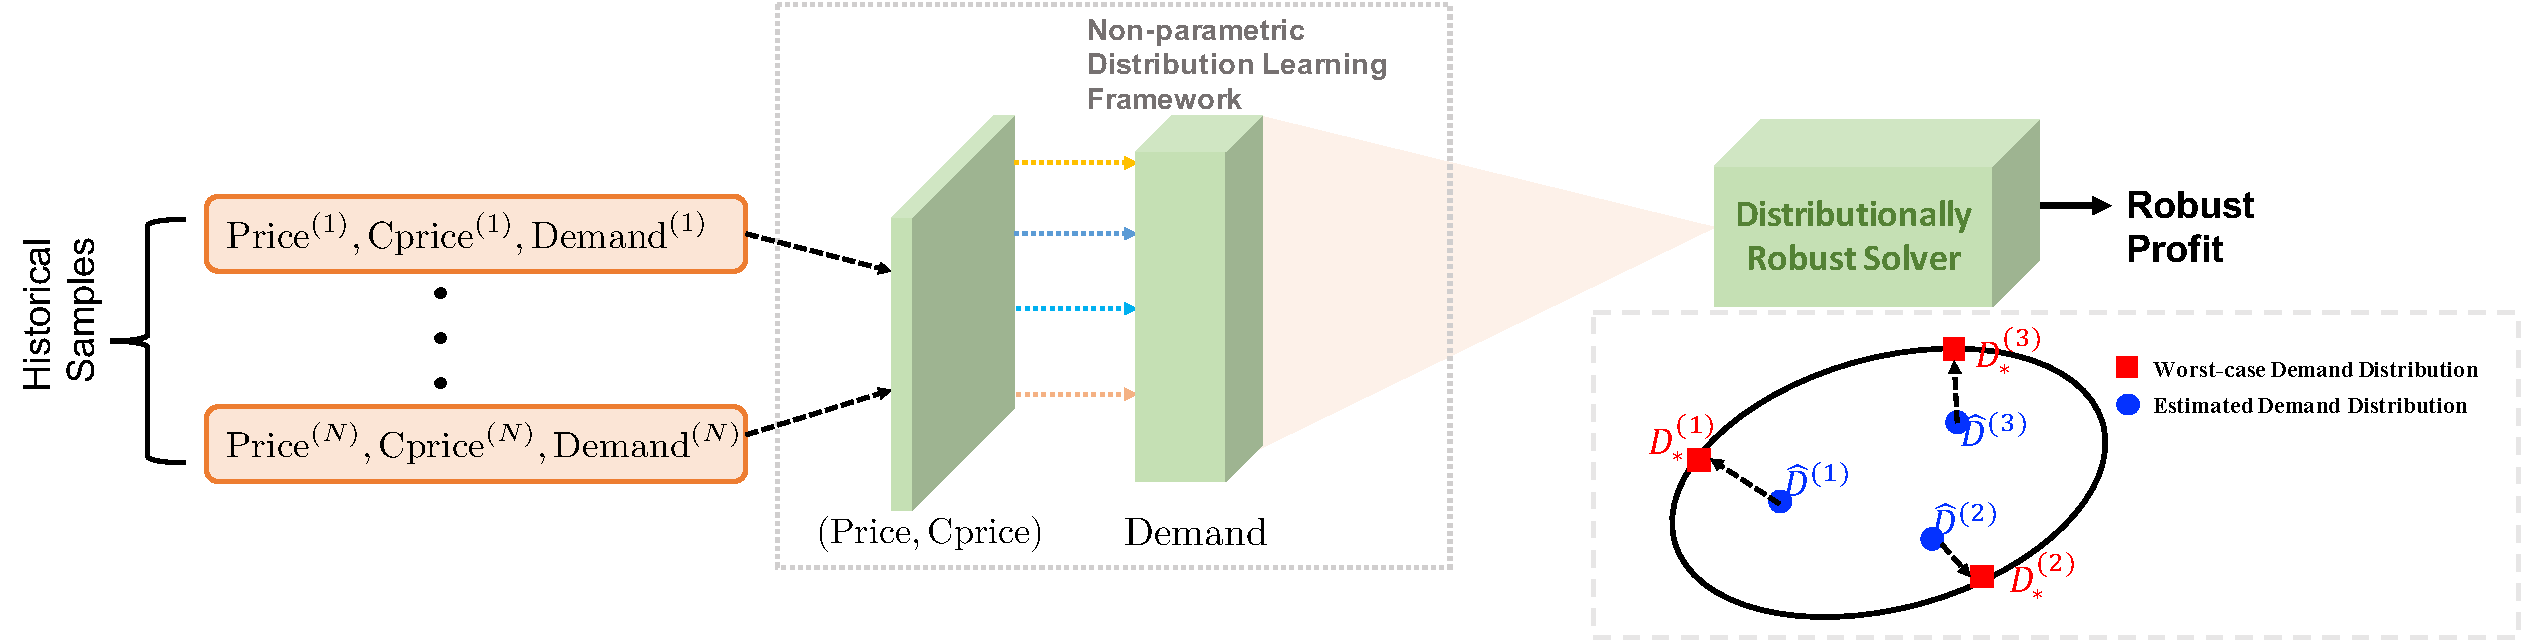
\includegraphics[width=0.8\textwidth]{diagram_0925_new.pdf}
    \caption{An overview of the proposed framework, which consists of two critical components: (a) a non-parametric framework that estimates the demand distribution based on historical samples; (b) a distributionally robust solver that estimates a robust profit based on the estimated demand distribution.}
    \vspace{-1em}
    \label{fig:diagram_0925}
\end{figure}



\vspace{-1em}
\section{Methodology}\label{Sec:method}
Consider a retailer who sells a single product with finite amount of inventory.
Assume the amount of inventory available for sale, denoted as $y\in\mathbb{R}_+$ is known to the retailer, and he/her determines the price $p\in[p^l, p^u]$ for sale.
%an unit price $p\in[p^l, p^u]$ for each product to sale.
Besides, the retailer is provided with the cprice~(i.e., competitors' price) $z\in \mathbb{R}^{M}$ with $M\in\mathbb{N}_+$, which can be viewed as a covariate variable.
Here we assume that the price decision $p$ and the cprice $z$ will influence the customer demand $D$ distribution, which follows the probability distribution $f_D(p, z)$.
%demand distribution, denoted as $D\sim f_D(p, z)$.
The goal is to select the optimal price such that the expected profit $\mathbb{E}_{D\sim f_D(p,z)}[c(p,D)]$ is maximized.
In the following, we provide the detailed expression regarding the profit function $c(p,D)$.

\noindent{\bf Profit Model.}
%\paragraph{Loss Model.}
It is known that the profit depends on \emph{sales}, \emph{Cost of Goods Sold}~(COGs), \emph{eCommerce Fee}~(FBA), \emph{Referral Fee}~(REFFEE), and \emph{Ad Spend}~(ADSPEND). 
Given the price $p$, customer demand $D$, and inventory level $y$, we know $\mathrm{sales}=p(D\land y)$.
We make the following assumption regarding the other four variables:
\vspace{-0.5em}
\begin{assumption}\label{Assumption:model}
% \begin{enumerate}
%     \item 
% $\mathrm{COGs} = a_1\cdot(D\land y)$;
% $\mathrm{FBA} = a_2\cdot(D\land y)$;
% $\mathrm{REFFEE} =15\%\cdot p(D\land y)$;
% $\mathrm{ADSPEND}$ is a constant independent of any other variable.
%     \item
% $\mathrm{REFFEE} =15\%\cdot p(D\land y)$.
%      \item
% $\mathrm{ADSPEND}$ is a constant independent of any other variable.
% \end{enumerate}
$\mathrm{COGs} = a_1\cdot(D\land y)$;
$\mathrm{FBA} = a_2\cdot(D\land y)$;
$\mathrm{REFFEE} =15\%\cdot p(D\land y)$;
$\mathrm{ADSPEND}$ is a constant independent of any other variable.
\end{assumption} 
\vspace{-0.5em}
Here, we validate these assumptions using the provided SKU dataset \texttt{File Folders SKU 21}.
It turns out that these models fit the data with the high confidence level.
Specifically, the coefficients $a_1=4.43965609, a_2=6.60097822$.
Based on Assumption~\ref{Assumption:model}, we re-write the loss function 
$c(p,D)=0.85\cdot p(D\land y) - (a_1+a_2)\cdot (D\land y) - \text{ADSPEND}.$
Consider the ideal case where the demand distribution $f_D(p,z)$ is exactly known for any price $p$ and cprice $z$, the profit maximization problem becomes\vspace{-0.5em}
%Provided that the demand distribution $f_D(p,z)$ is exactly known for any price $p$ and covariat $z$, the profit maximization problem becomes
%Therefore, the profit maximization problem with known demand distribution becomes
\begin{equation}\label{Eq:true:loss}
\tag{Ideal}
\max_{p\in[p^l, p^u]}~\mathbb{E}_{D\sim f_D(p,z)}\Big[ 
0.85\cdot p(D\land y) - (a_1+a_2)\cdot (D\land y) 
\Big] - \mathrm{ADSPEND}.\vspace{-0.5em}
\end{equation}
%$c(p,D)=0.85\cdot p(D\land y) - (a_1+a_2)\cdot (D\land y) - \mathrm{ADSPEND}$.
In a practical case, one may not have full information regarding the inventory level $y$, the cprice~(i.e., competitors' prices) $z$, the variable $\mathrm{ADSPEND}$, and the demand distribution $f_D(p,z)$.
To tackle this challenge, we make the following simplifications:

%  \begin{minipage}{.55\textwidth}
\begin{itemize}
    \item 
We find in most situations, the inventory level $y$ is always greater than the units ordered, which motivates us to assume that $D\ll y$.
Thereby one can replace $D\land y$ with $y$ in problem~\eqref{Eq:true:loss}.
    \item
The cprice $z$ can be estimated using historical data based on time series prediction (e.g., based on python package \texttt{Skforecast}).
\end{itemize}

\begin{itemize}
    \item
From Figure~\ref{fig:adspend}, we find the variable $\mathrm{ADSPEND}$ seems to be correlated with variable $\mathrm{unitsordered}$.
Therefore, we estimate its value using time series prediction and treating variable $\mathrm{unitsordered}$ as an exogenous feature.
\item
The demand distribution $f_D(p,z)$ is difficult to obtain. In the following, we provide a non-parametric and data-driven way for estimating $f_D(p,z)$.% based on the collected data.
\end{itemize}

    
 
%\end{minipage}


    




% %In practice, we assume the inventory level $y$, covariate (i.e., competitors' prices) $z$, and constant $\mathrm{ADSPEND}$ are given.
% For example, with the given dataset, one can estimate $y, z, \mathrm{ADSPEND}$ based on time series prediction using historical data.
% From the plot in Figure~\ref{fig:adspend}, we find the variable $\mathrm{ADSPEND}$ seems to be correlated with $\mathrm{unitsordered}$.
% So we predict the future value of $\mathrm{ADSPEND}$ based on historical data of $\mathrm{ADSPEND}$ and $\mathrm{unitsordered}$ jointly.
% \begin{figure}[t]
%     \centering
%     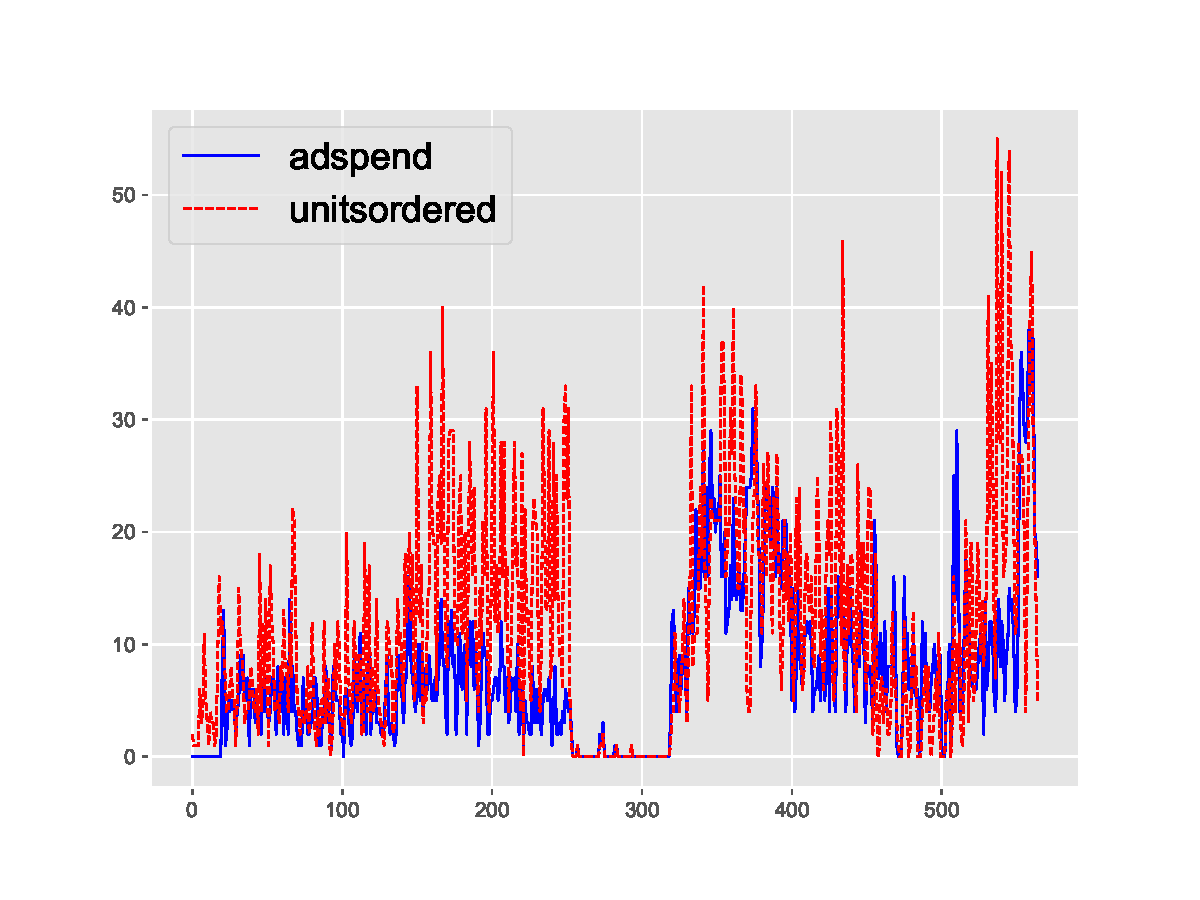
\includegraphics[width=0.5\textwidth]{adspend_units.pdf}
%     \caption{Plot of adspend and units of order versus time index}
%     \label{fig:adspend}
% \end{figure}
%However, the demand distribution $f_D(p,z)$ is usually not available.
%In the following, we provide a non-parametric and data-driven way for estimating $f_D(p,z)$ based on the collected data.
\begin{wrapfigure}{r}{0.3\textwidth}
\vspace{-2em}
\centering
\captionsetup{justification=raggedright}
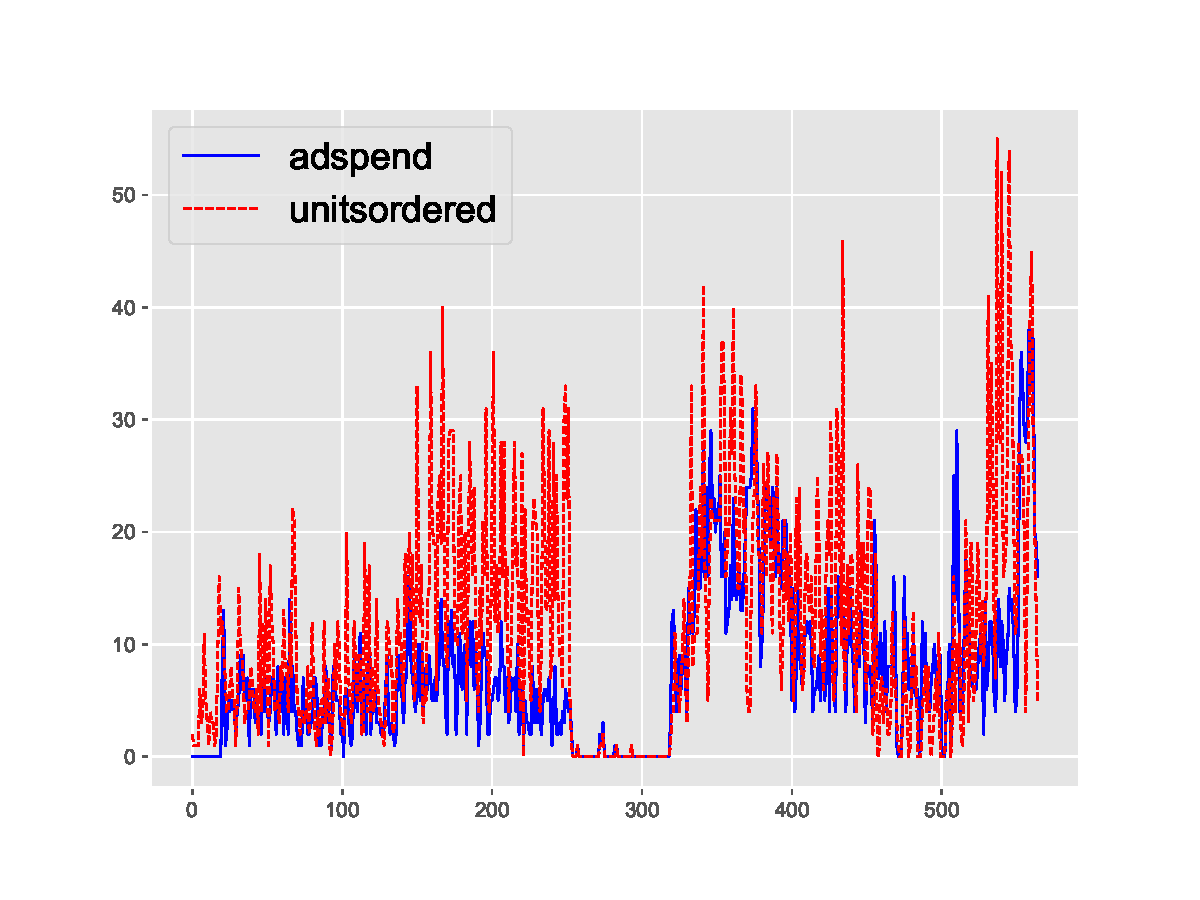
\includegraphics[width=0.3\textwidth]{adspend_units.pdf}
 \caption{{\rmfamily Plot of $\mathrm{ADSPEND}$ and $\mathrm{Unitsordered}$ versus time index for product \texttt{File Folders SKU 21}}.}
\label{fig:adspend}
\vspace{-3em}
\end{wrapfigure}
\noindent 
{\bf Demand Distribution.}
We provide a data-driven estimation of the demand distribution $f_D(p,z)$, in which only data samples $\{(p^i, z^i, D^i)\}_{i=1}^N$ are available. 
For a given price-cprice pair $(p,z)$, we approximate the true demand distribution using the weighted discrete distribution sharing the same support of the training dataset:
\[\small
\widehat{\mathbb{P}}_n^{(p,z)} = \sum_{i=1}^N\omega^i(p,z)\delta_{D^i},
\]
where the weight function $\{\omega^i(p,z)\}_{i=1}^N$ are obtained using the (Gaussian) kernel regression model:
\vspace{-1.5em}
\begin{equation}\label{Eq:KR:model}
\omega^i(p,z)\propto \exp\left( 
\frac{-\|(p,z) - (p^i,z^i)\|_2^2}{2\sigma^2}
\right),\quad 
\sum_{i=1}^N\omega^i(p,z)=1.\vspace{-0.5em}
\end{equation}
%$k$-nearest neighbor model.
%random forest model following techniques from the existing literature~\citep{bertsimas2020predictive}.
Previous studies have proposed several modeling for customer demand, such as additive linear model~\citep{wang2015optimal, bu2022context} and multiplicative model~\citep{kazaz2015price, salinger2011simple}. However, it is vague whether those models result in an accurate estimation of the demand in our setting because the cprice $z$ is involved. 
Instead, we use a data-driven estimator in this part, which is quite flexible as we \emph{'let the data speak for itself.'}


\noindent 
{\bf Distributionally Robust Formulation.}
A natural pricing idea is to solve the sample average approximation~(SAA) counterpart of problem~\eqref{Eq:true:loss}, i.e., by replacing $f_D(p,z)$ with the estimated distribution $\widehat{\mathbb{P}}_n$ and solve the approximated problem.
However, SAA may not achieve satisfactory performance because the estimate $\widehat{\mathbb{P}}_n$ is not accurate enough.
Instead, we solve the distributionally robust counterpart of the SAA problem using the %KL-divergence 
$2$-Wasserstein distance
to model the ambiguity set:
\begin{equation}
\label{Eq:DRO:pricing}
\tag{DRO-Pricing}
\max_{p\in[p^l, p^u]}~\left\{\min_{ \mathbb{P}:~\mathrm{supp}(\mathbb{P})\subseteq \mathrm{supp}(\widehat{\mathbb{P}}_n^{(p,z)})}~\mathbb{E}_{D\sim \mathbb{P}}[c(p,D)]:~
\mathcal{W}\left(\mathbb{P},\widehat{\mathbb{P}}_n^{(p,z)}\right)\le \epsilon
\right\}.
\end{equation}
Here the $2$-Wasserstein distance is defined as
\[\small
\mathcal{W}(\mathbb{P}, \mathbb{Q}):=\min_{\gamma}~\left\{ 
\big(\mathbb{E}[\|\omega - \omega'\|^2]\big)^{1/2}:~
\begin{array}{l}
\text{$\gamma$ is a joint distribution of $(\omega,\omega')$}\\
\text{with mariginal distributions $\mathbb{P}$ and $\mathbb{Q}$}
\end{array}
\right\}.
\]
% \[
% \max_{p\in[p^l, p^u]}~\left\{\min_{ \mathbb{P}:~\mathrm{supp}(\mathbb{P})\subseteq \mathrm{supp}(\widehat{\mathbb{P}}_n^{(p,z)})}~\mathbb{E}_{D\sim \mathbb{P}}[c(p,D)]:~
% \mathcal{W}\left(\mathbb{P},\widehat{\mathbb{P}}_n^{(p,z)}\right)\le \epsilon
% \right\}.
% \]
For fixed price $p$ and cprice $z$, according to the definition of Wasserstein distance, the inner minimization problem can be reformulated as a linear program that can be solved efficiently:
\begin{equation}\label{Eq:LP:pricing}
\min_{\gamma\in\mathbb{R}^{N\times N}, \nu\in\mathbb{R}^N_+}~\left\{ 
\sum_{i=1}^N\nu_ic(p, D^i):~
\left\{ 
\begin{array}{l}
\sum_{i=1}^N\gamma_{i,j}=\nu_j, \forall j, \sum_{j=1}^N\gamma_{i,j}=\omega^i(p,z),\forall i,\\
\sum_{i,j=1}^N\gamma_{i,j}|D^i - D^j|^2\le \epsilon^2
\end{array}
\right\}
\right\}.
\end{equation}
It is worth mentioning that \eqref{Eq:DRO:pricing} is a nonconvex optimization problem because the decision variable $p$ influences both the objective function and the demand distribution.
However, it is required that the optimized pricing value should end in $0.05$ or $0.09$.
Therefore, we solve problem~\eqref{Eq:DRO:pricing} by enumerating all possible choices of price $p$, whereas for each value $p$ one only needs to solve a linear programming formulation~\eqref{Eq:LP:pricing}.
Similarly, one can obtain an optimistic pricing strategy by replacing the inner minimization in problem~\eqref{Eq:DRO:pricing} with maximization.

\begin{remark}[The Spirit of Robustness]
By solving problem~\eqref{Eq:DRO:pricing}, the retailer tends to find a price to maximize his/her profit under the worst scenario among all customer demand distributions. 
Even if the true demand distribution is shifted slightly compared to the estimated demand distribution due to the dynamic market environment, a distributionally robust pricing strategy could still provide a lower bound on the actual profit.
On the supply side, there is less room for the retailer to make a wrong pricing strategy with limited information on the demand distribution because of the marginal cost.
Therefore, a distributionally robust strategy seems preferable.
%due to the marginal cost, there is less room for the retailer to make a wrong pricing strategy 
\end{remark}
% \begin{remark}[Selection of Hyper-parameters]
% The bandwidth parameter $\sigma^2$ in \eqref{Eq:KR:model} and the radius of ambiguity set $\epsilon$ in \eqref{Eq:DRO:pricing} plays a critical impact on the performance of our model.
% We tune these two hyper-parameters using cross-validation: we split the given dataset into the training and validation sets. For each candidate pair $(\sigma^2,\epsilon)$, we formulate the estimated profit for each sample in the validation set based on the training set.
% Then, we take the optimal hyper-parameter as the one that achieves the smallest residual error between the estimated profit and the true profit in the validation set. 
% \end{remark}

%\section{Algorithm}
\vspace{-1em}
\section{Numerical Study}

The bandwidth parameter $\sigma^2$ in \eqref{Eq:KR:model} and the radius of ambiguity set $\epsilon$ in \eqref{Eq:DRO:pricing} plays a critical impact on the performance of our model.
In our numerical study, we tune these hyper-parameters using cross-validation: we split the given dataset into the training and validation sets. For each candidate pair $(\sigma^2,\epsilon)$, we formulate the estimated profit for each sample in the validation set based on the training set.
Then, we take the optimal hyper-parameter as the one that achieves the smallest residual error between the estimated profit and the true profit in the validation set. 
\subsection{Profit Estimation}
\begin{wrapfigure}{r}{0.25\textwidth}
\vspace{-6em}
\centering
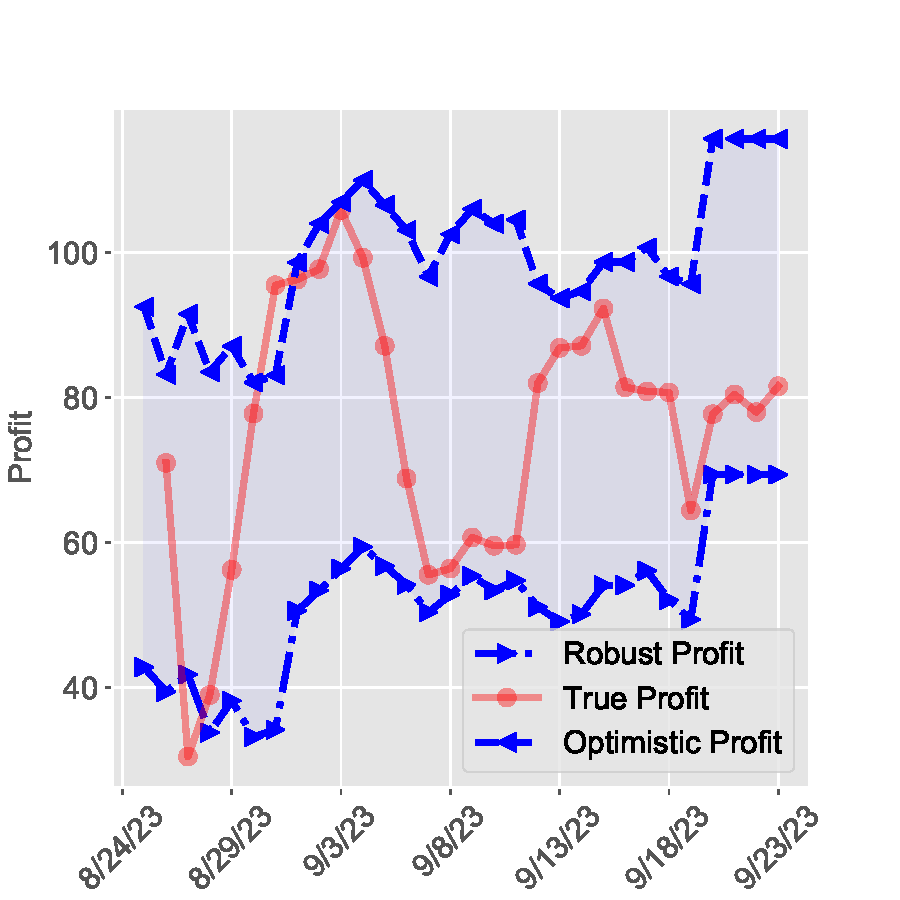
\includegraphics[width=0.25\textwidth]{Profit_estimator.pdf}
\vspace{-2em}
 \caption{Plot of estimated profit versus true profit in last 30 days.}
 \vspace{-2em}
\label{fig:profit:estimate}
%\vspace{-3em}
\end{wrapfigure}
We use the historical data from the last $30$ days as the testing data and use the remaining data as the training data to examine the performance of our profit estimation algorithm.
Figure~\ref{fig:profit:estimate} reports the plot of true expected profit~\footnote{
We take the average of profit within the nearest $7$ days as the true expected profit.
} together with estimated robust and optimistic profit.
%robust/optimistic profit based on true covariate and ADSPEND inputs, and robust/optimistic profit based on estimated covariate and ADSPEND inputs.
From the plot, we find our profit estimation algorithm works reasonably well: the true profit is generally covered by $[\text{robust profit}, \text{optimistic profit}]$ with a reasonably tight interval width.

\subsection{Visualization of Demand Distribution}
Next, we visualize the estimated robust demand distribution for various price choices and fix the cprice $z=22.99$ by treating the provided dataset as the training set.
See the visualization in Figure~\ref{fig:price:demand}.
From the plot, we find that customer demand tends to decrease as the price value increases, which is consistent with our intuition.
\begin{figure}[H]
\vspace{-1.8em}
    \centering
    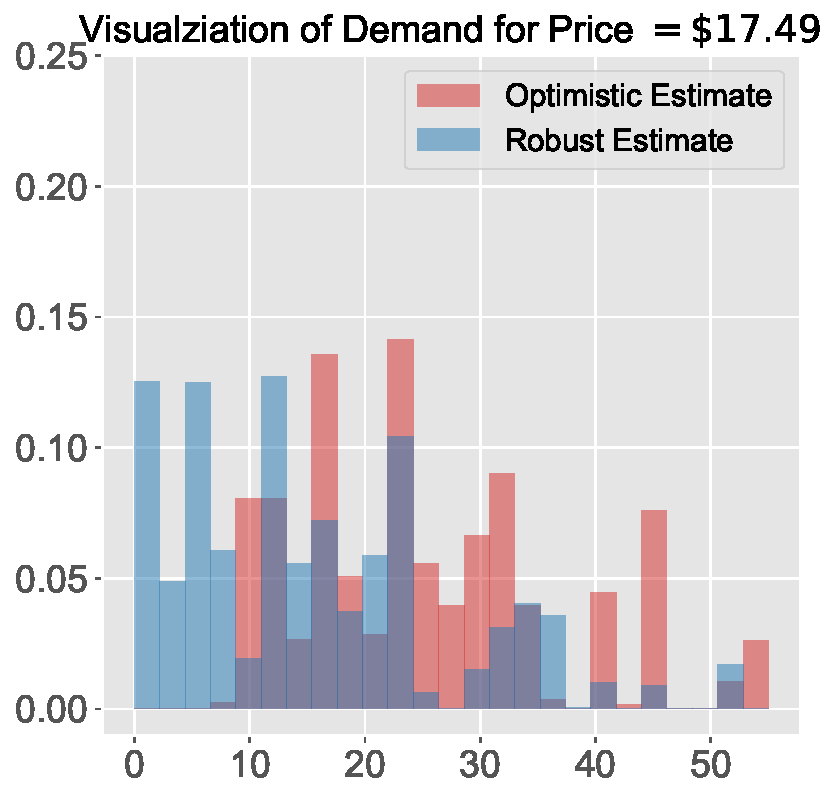
\includegraphics[width=0.19\textwidth]{Plot_Histogram_Demand_1.pdf}
    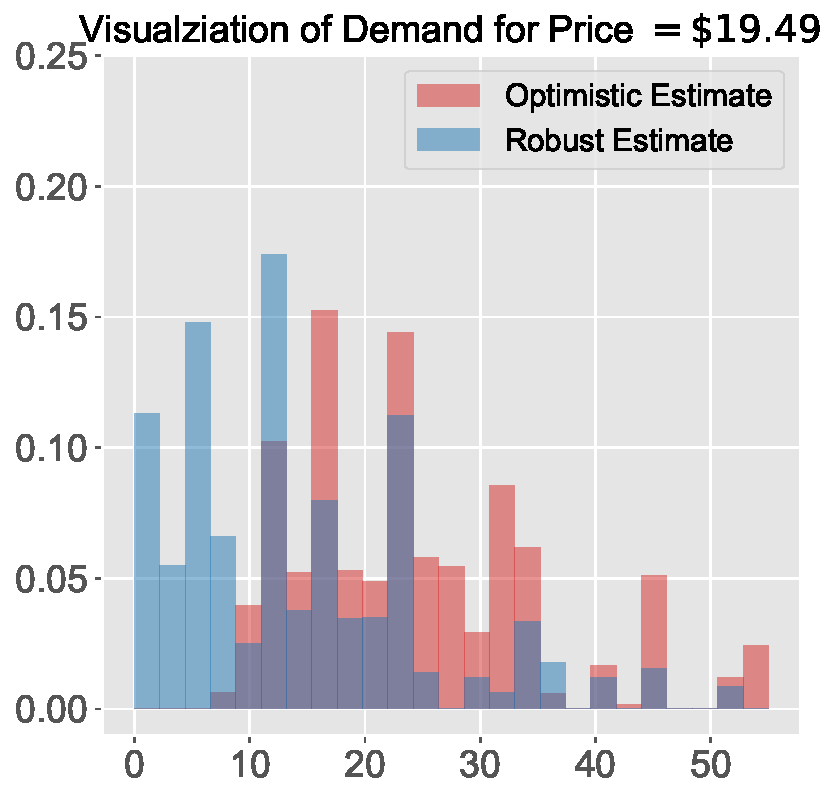
\includegraphics[width=0.19\textwidth]{Plot_Histogram_Demand_2.pdf}
    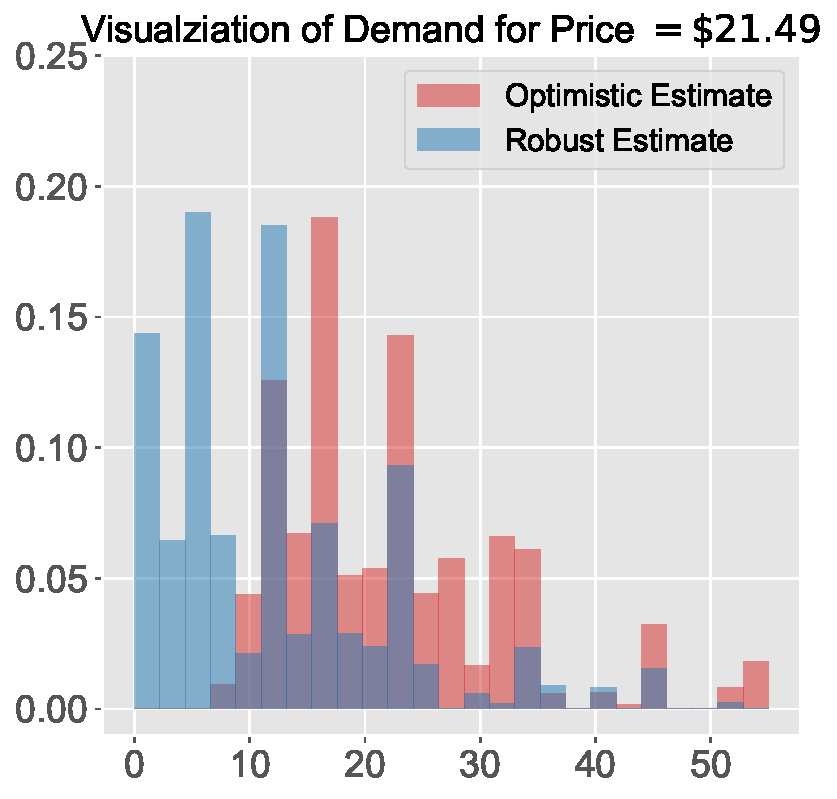
\includegraphics[width=0.19\textwidth]{Plot_Histogram_Demand_3.pdf}
    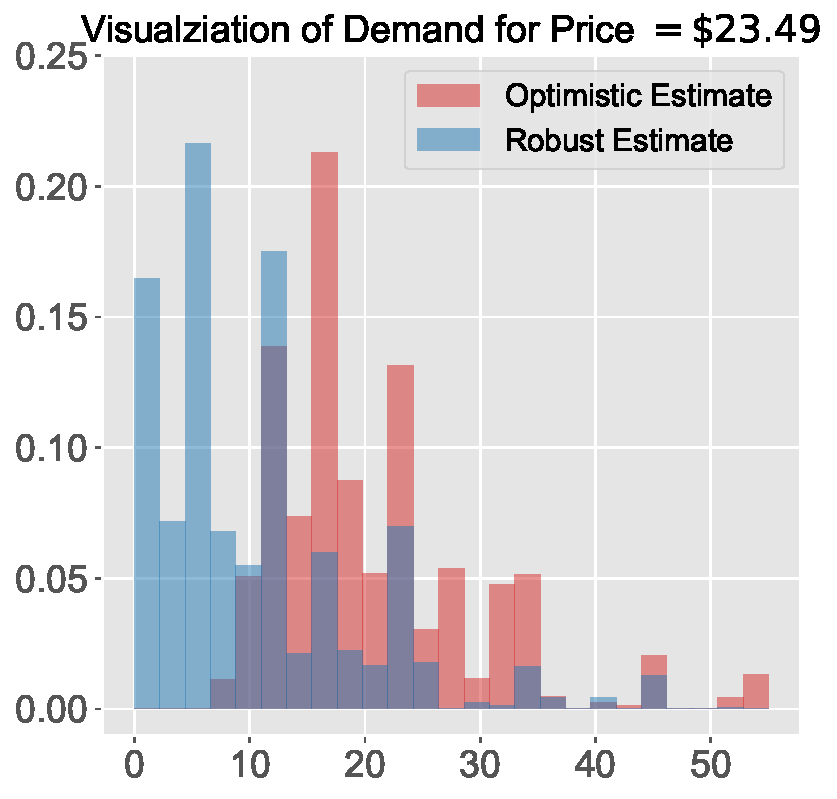
\includegraphics[width=0.19\textwidth]{Plot_Histogram_Demand_4.pdf}
    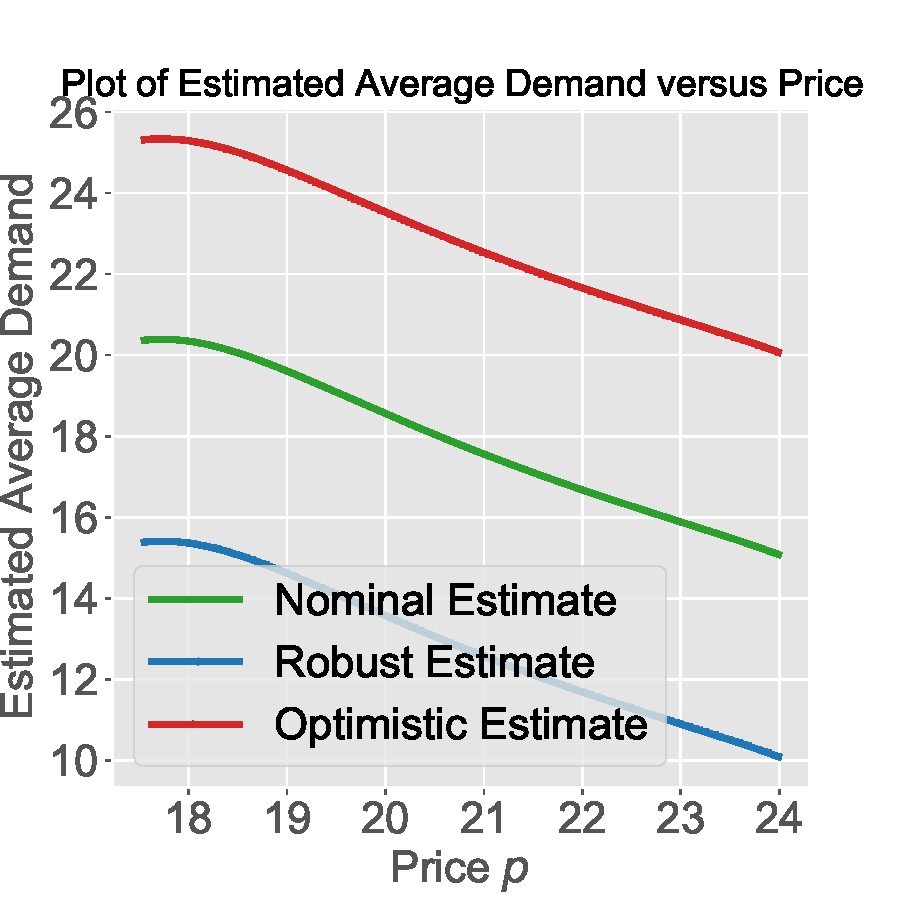
\includegraphics[width=0.19\textwidth]{demand_summary.pdf}
    \caption{The four left plots visualize the estimated demand distribution for different prices. The rightmost plot reports the estimated \emph{average} demand across different choices of price.}
    \label{fig:price:demand}
    \vspace{-2em}
\end{figure}
%customer demand tends to decrease as the price value increases, which is consistent with our intuition. 



\subsection{Optimal Pricing}
\begin{wrapfigure}{r}{0.48\textwidth}
\vspace{-4em}
\centering
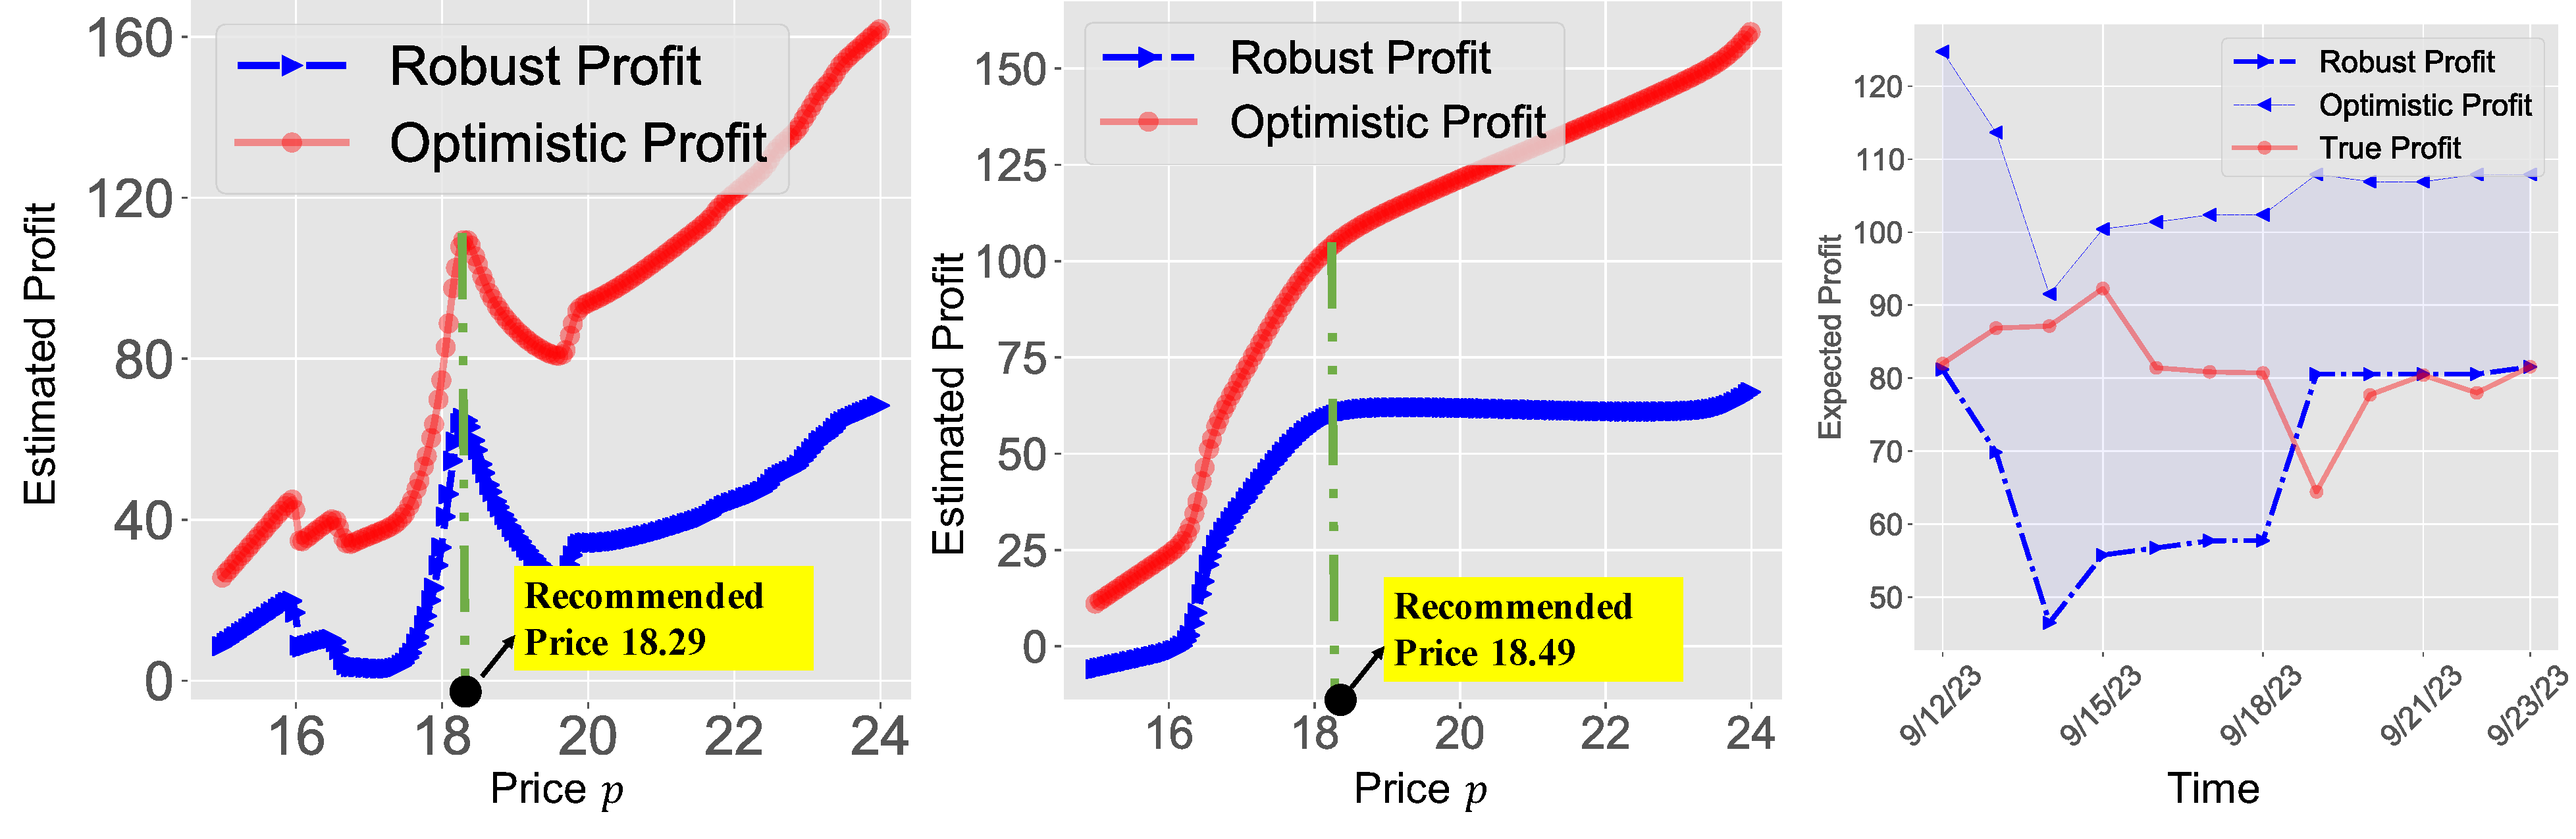
\includegraphics[width=0.45\textwidth]{Pricing_summary.pdf}
% \includegraphics[width=0.15\textwidth]{price_week1_updated.pdf}
% \includegraphics[width=0.15\textwidth]{price_week1_updated.pdf}
%\vspace{-2em}
 \caption{Left two: estimated profit for different prices during Week~1/Week~2 testing phase; Right: Estimated profit v.s. true profit.}
 \vspace{-2em}
\label{fig:profit:summary}
%\vspace{-3em}
\end{wrapfigure}
Finally, we present the average of estimated profits across different price choices for Week~1~(Sep.12-18) and Week~2~(Sep.19-25) in Figure~\ref{fig:profit:summary}.
From the plots, we realize that price $23.99$ results in the best robust profit, but its interval width~(optimistic profit minus robust profit) is also the largest, indicating it is not a stable and robust choice.
Instead, we prefer to take a price that results in (nearly) the best robust profit but with a significantly small interval width. 
Therefore, we take the price $18.29$ in Week~1 and price $18.49$ in Week~2.
Figure~\ref{fig:profit:summary}(c) plots the estimated profit and true profit during these two weeks, from which we can see that the numerical performance of our pricing and profit estimation strategy works reasonably well.






\vspace{-1em}
\section{Conclusion}
We develop a data-driven pricing strategy that not only yields an optimal price but also provides interval estimation of the expected profit.
Its practical performance on the \texttt{File Folders SKU 21} product has the second-highest rank among all File Folders SKU products, as validated by official rankings.

\vspace{-1em}
\section{Team Member(s)}

%List all team members associated with the submission, including the corresponding author. A team’s solution should be submitted once (as opposed to each member of the team submitting the same solution individually).

\begin{itemize}
\item Jie Wang, Georgia Institute of Technology, Atlanta, GA 30332, jwang3163@gatech.edu
%\item Team Member 2, Affiliation and address, TM2@email.com
%\item Team Member 3, Affiliation and address, TM3@email.com
\end{itemize}




% In the formulation above, it is assumed that inventory level $z$

% %maximize the profit $\mathbb{E}_{D\sim f_D(p,z)}[c(p,D)]$


% %in the face of a finite amount of inventory. 

% In the following, we discuss our estimated model based on dataset.
% \subsection{Market Demand}
% It seems that the market demand $d$ for the product is influenced by the price $p$ and the prices from potential competitors, denoted as $\tilde{\mathbf{p}}\in\mathbb{R}^{M}$ with $M\in\mathbb{N}_+$.
% We have available data samples $\{(d^{(i)}, p^{(i)}, \tilde{\mathbf{p}}^{(i)})\}_{i\in[N]}$, from which we can infer the relation between the market demand $d$ and the price vector $(p, \tilde{\mathbf{p}})$.
% We pre-process the data samples by taking
% \[
% x = 2\cdot\frac{ p - \min_ip^{(i)}}{\max_ip^{(i)} - \min_ip^{(i)}}-1\in[-1,1],\qquad 
% \tilde{\mathbf{x}} = 2\cdot\frac{\tilde{\mathbf{p}}- \min_i\tilde{\mathbf{p}}^{(i)}}{\max_i\tilde{\mathbf{p}}^{(i)} - \min_i\tilde{\mathbf{p}}^{(i)}}-1\in[-1,1]^M.
% \]
% Then we propose the following linear model of the market demand:
% \[
% d = \zeta + \beta_0x + 
% \sum_{i\in[M]}~\beta_i\tilde{\mathbf{x}}_i
% +
% \sum_{i\in[M]}\alpha_{0,i}x\tilde{\mathbf{x}}_i
% +
% \sum_{i\in[M]}
% \sum_{j=i+1}^M
% \alpha_{i,j}\tilde{\mathbf{x}}_i\tilde{\mathbf{x}}_j,
% \]
% where the model parameters $\theta:=(\beta_{0},\beta_i,\alpha_{0,i}, \alpha_{i,j})\in \mathbb{R}^{2M+1+M(M-1)/2}$ can be estimated based on data.




% %where the operators on the second  

% %This motivates us to propose the following linear model





% We make the following assumption regarding the demand for the product.
% \begin{assumption}
% The market demand for the product with the price set to $p$ is 
% \[
% \mathcal{D}(p) = \zeta - b_1p - b_2(p-p_{\mathrm{other}}).
% \]
% Here $p_{\mathrm{other}}$ denotes the minimum price among all competitors for a similar product.
% If this information is not available in practice, we set $p_{\mathrm{other}} = p$.
% \end{assumption}
% Besides, the profit also depends on \emph{Cost of Goods Sold}~(COGs), \emph{eCommerce Fee}~(FBA), \emph{Referral Fee}~(REFFEE), and \emph{Ad Spend}~(ADSPEND). 
% We make the following assumption regarding the first three factors:
% \begin{assumption}
% \begin{enumerate}
%     \item 
% $\mathrm{COGs} = a_1\cdot \mathrm{demand}$.
%     \item
% $\mathrm{FBA} = a_2\cdot \mathrm{demand}$.
%     \item
% $\mathrm{REFFEE} =85\%\cdot\mathrm{sales}$.
% \end{enumerate}
% \end{assumption}
% It seems that the variable ADSPEND is independent of all other variables except time. 
% We model its value as a time series and use auto-regressive model to predict its value.
% In summary, the goal is to find an optimal price $p^*$ such that the profit objective is maximized, i.e., 
% \[
% p^* = \argmax_{p\in[p^l, p^u]}~\Big\{ 
% F(p)\triangleq \mathrm{Sales}
% %p\cdot\bE[\min\{\mathcal{D}(p), y\}]
% - \mathrm{COGs} - 
% \mathrm{FBA} - \mathrm{REFFEE} - \mathrm{ADSPEND}
% \Big\},
% \]
% where the objective can be re-written as
% \[
% F(p) = 
% 85\%\cdot p\cdot\bE[\min\{\mathcal{D}(p), y\}] - (a_1+a_2)\bE[\mathcal{D}(p)] - \mathrm{ADSPEND}.
% \]
% In particular, the hyper-parameters $a_1,a_2,b_1,b_2,\mathrm{ADSPEND}$ are estimated based on offline data: coefficients $a_1$ and $a_2$ can be estimated using the linear regression technique, $\mathrm{ADSPEND}$ can be estimated using common methods in time series prediction.

% In the following, we discuss how to obtain the price sensitivity parameters $b_1$ and $b_2$.




\vspace{-1em}
\bibliographystyle{informs2014} 
{
\footnotesize
\bibliography{shortbib}
}




%\appendices

\end{document}